\section{Non-interactive blockchain \emph{infix} proofs}
\label{sec:infix}

In the previous section we have seen how to construct proofs for suffix
predicates. As mentioned, the main purpose of that construction is to serve as a
stepping stone for the construction of this section that presents a more useful
class of proofs. This class of proofs allows proving more general predicates
that can depend on multiple blocks even buried deep within the blockchain.

More specifically, the generalized prover for \emph{infix proofs} allows
proving any predicate $Q(\chain)$ that depends on a number of blocks that can
appear anywhere within the chain (except the $k$ suffix for stability). These
blocks constitute a \emph{subset} $\chain'$ of blocks, the \emph{witness},
which may not necessarily form a chain. This allows proving useful statements
such as, for example, whether a transaction is confirmed. We next formally
define the class of predicates that will be of interest.

% XXX extend this class of predicates to include comparison of position
% within the blockchain (these position-dependent predicates may be unprovable
% in velvet mode due to diamond topologies)
\begin{definition}[Infix sensitivity]
\label{def:infix}
A chain predicate $Q_{d,k}$ is \textnormal{infix sensitive} if it can be
written in the form

$$
Q_{d,k}(\chain) =
\begin{cases}
  \text{\emph{true}, if }
    \exists \chain' \subseteq \chain[:-k]: |\chain'| \leq d \land D(\chain')\\
  \text{\emph{false}, otherwise}
\end{cases}
$$

where $D$ is an arbitrary efficiently computable predicate.
\end{definition}

Note that $\chain'$ is a blockset and may not necessarily be a blockchain.
Furthermore, observe that for all blocksets $\chain' \subseteq \chain$ we have
that $Q(\chain') \Rightarrow Q(\chain)$. This will allow us to later argue that
adding more blocks to a blockchain cannot invalidate its witness.

Similarly to suffix-sensitive predicates, infix-sensitive predicates $Q$ can be
evaluated very efficiently. Intuitively this is possible because of their
localized nature and dependency on the $D(\cdot)$ predicate which requires only
a small number of blocks to conclude whether the predicate should be true.

\noindent\textbf{Example.}
We next show how to express the predicate that asks whether a certain
transaction with id $txid$ has been confirmed as an infix sensitive predicate.
We define the predicate $D^{txid}$ that receives a single block and tests
whether a transaction with id $txid$ is included. The predicate $Q^{txid}_{1,
k}$ is defined as in Definition~\ref{def:infix} using the predicate $D^{txid}$
and the parameter $k$ which in this case determines the desired stability of the
assertion that $txid$ is included (e.g., $k = 6$). $Q$ alone proves that a
particular block is included in the blockchain. Some auxiliary data is supplied
by the prover to aid the provability of transaction inclusion: the Merkle Tree
proof-of-inclusion path to the transactions Merkle Tree root, similar to an SPV
proof. This data is logarithmic in the number of transactions in the block and,
hence, constant with respect to blockchain size. In case of a vendor awaiting
transaction confirmation to ship a product, the proof that a certain transaction
paid into a designated address for the particular order is sufficient. In this
scheme it is impossible to determine whether the money has subsequently been
spent in a future block, and so must only be used by the vendor holding the
respective secret keys.

In the above example, note that if the verifier outputs \emph{false}, this
behavior will generally be inconclusive in the sense that the verifier could be
outputting \emph{false} either because the payment has not yet been confirmed or
because the payment was never made.
% We can easily modify the scheme to allow the
% payer to claim that the payment was made at some particular block height $\ell$.
% The vendor can then bail out after a number of blocks $\ell$ and conclude that
% the payment was never made. In order to do that formally, \emph{two} different
% infix predicates must be evaluated by the NIPoPoW protocol. The first predicate
% $Q_1$ as above simply checks for transaction confirmation. The second predicate
% $Q_2$ attests to the size of the underlying blockchain and in particular returns
% \emph{true} if the blockchain has grown beyond $\ell$ blocks long. The payment
% is deemed successful if $Q_1$ outputs \emph{true} and unsuccessful if $Q_2$
% outputs \emph{true}. While both predicates are \emph{false} the result of the
% experiment is inconclusive. The predicate $Q_2$ can be implemented in
% blockchains which include a verified block height in their block headers such as
% Ethereum. As always, the block whose header is checked for block height must be
% a \emph{stable} block in $\chain[:-k]$ to ensure that a malicious miner is not
% able to tamper with it.

\begin{figure}[h]
    \caption{An infix proof descend. Only blue blocks are included in the proof.
    Blue blocks of level $4$ are part of $\pi$, while the blue blocks of level
    $1$ through $3$ are produced by followDown to get to the block of level $0$
    which is part of $\chain'$.}
    \centering
    \iftwocolumn
        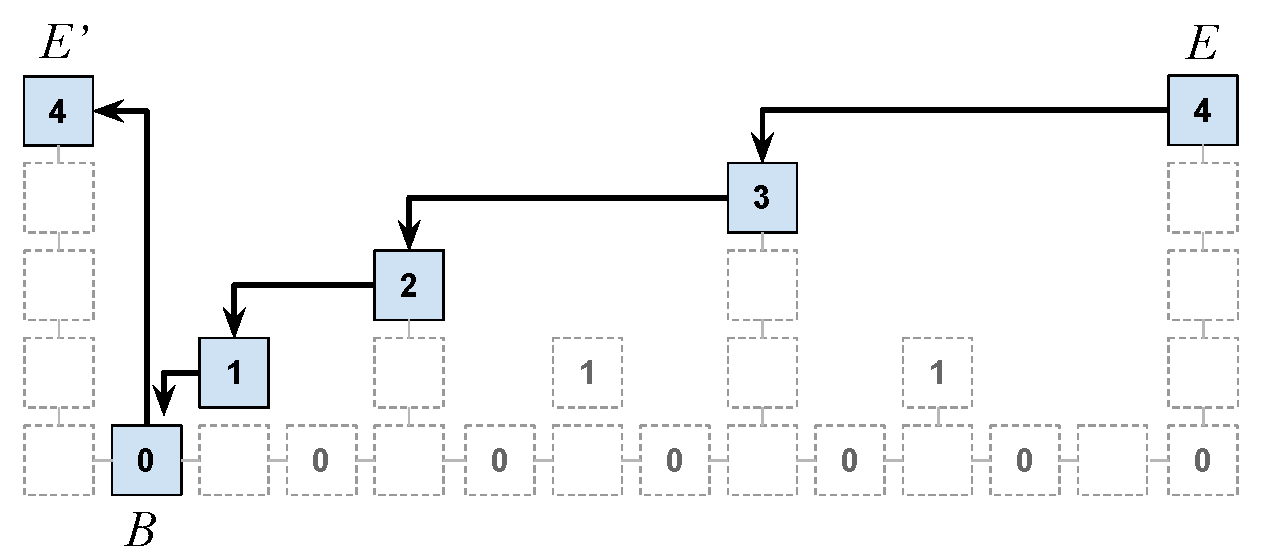
\includegraphics[width=0.9\columnwidth,keepaspectratio]{figures/infix.pdf}
    \else
        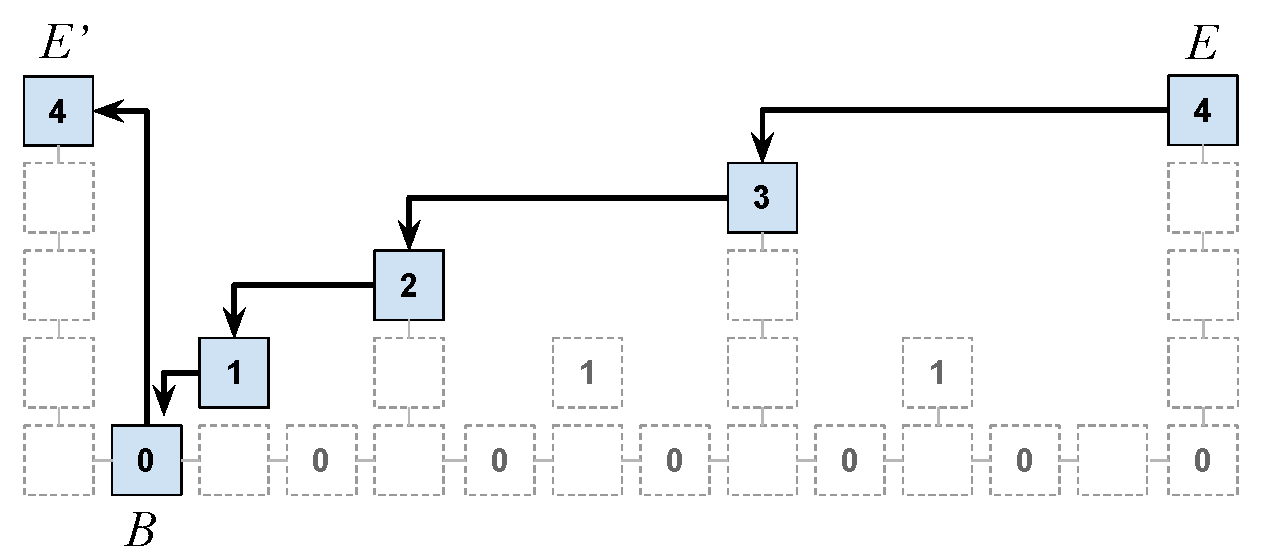
\includegraphics[width=0.7\columnwidth,keepaspectratio]{figures/infix.pdf}
    \fi
    \label{fig.infix}
\end{figure}

\subsection{Construction}

The construction of these proofs is shown in
Algorithm~\ref{alg.nipopow-infix-prover}. The infix prover accepts two
parameters: The chain $\chain$ which is the full blockchain and $\chain'$ which
is a sub-blockset of the blockchain and whose blocks are of interest for the
predicate in question. The prover calls the previous suffix prover to produce a
proof as usual. Then, having the prefix $\pi$ and suffix $\chi$ of the suffix
proof in hand, the infix prover adds a few auxiliary blocks to the prefix $\pi$.
The prover ensures that these auxiliary blocks form a chain with the rest of the
proof $\pi$. Such auxiliary blocks are collected as follows: For every block $B$
of the subset $\chain'$, the immediate previous ($E'$) and next ($E$) blocks
in $\pi$ are found. Then, a chain of blocks $R$ which connects $E$ back to $B$
is found by the algorithm \textsf{followDown}. If $E'$ is of level $\mu$, there
can be no other $\mu$-superblock between $B$ and $E'$, otherwise it would have
been included in $\pi$. Therefore, $B$ already contains a pointer to $E'$ in its
interlink, completing the chain.

\import{./}{algorithms/alg.nipopow-infix-prover.tex}

The way to connect a superblock to a previous lower-level block is implemented
in Algorithm~\ref{alg.nipopow-infix-follow}.  Block $B'$ cannot be of higher or
equal level than $E$, otherwise it would be equal to $E$ and the
\textsf{followDown} algorithm would return. The algorithm proceeds as follows:
Starting at block $E$, it tries to follow a pointer to as far as possible. If
following the pointer surpasses $B$, then the procedure at this level is aborted
and a lower level is tried, which will cause a smaller step within the skiplist.
If a pointer was followed without surpassing $B$, the operation continues from
the new block, until eventually $B$ is reached, which concludes the algorithm.

\import{./}{algorithms/alg.nipopow-infix-follow.tex}

An example of the output of \textsf{followDown} is shown in
Figure~\ref{fig.infix}. This is a portion of the proof shown at the point where
the superblock levels are at level $4$. A descend to level $0$ was necessary so
that a regular block would be included in the chain. The level $0$ block can
jump immediately back up to level $4$ because it has a high-level pointer.

The verification algorithm must then be modified as in
Algorithm~\ref{alg.nipopow-verifier-infix}.

The algorithm works by calling the suffix verifier. It also maintains a blockDAG
collecting blocks from all proofs (it is a DAG because \textit{interlink} can be
adversarially defined in adversarially mined blocks). This DAG is maintained in
the $\textsf{blockById}$ hashmap. Using it, \textsf{ancestors} uses simple graph
search to extract the set of ancestor blocks of a block. In the final predicate
evaluation, the set of ancestors of the best blockchain tip is passed to the
predicate. The ancestors are included to avoid an adversary who presents an
honest chain but skips the blocks of interest. In particular, such an adversary
would work by including a complete suffix proof, but ``forgetting'' to include
the blocks generated by \textsf{followDown} for the infix proof pertaining to
blocks in $\chain'$.

\import{./}{algorithms/alg.verifier-infix.tex}
